\NeedsTeXFormat{LaTeX2e}
%-----------------------------------------------------------
\documentclass[a4paper,12pt]{monografia}
\usepackage[alf]{abntex2cite}
\usepackage[brazil]{babel}
\usepackage[utf8]{inputenc}
\usepackage{indentfirst}
\usepackage{url}
\usepackage{amsmath}

\usepackage{subfig}
\usepackage{graphicx}

%\usepackage[hidelinks]{hyperref}
%-----------------------------------------------------------
\begin{document}

\pagenumbering{roman}
%-----------Título e Dados do Autor---------------------------
\titulo{Reconstrução de Objetos 3D a partir de Imagens 2D}
%\subtitulo{Subtítulo} % opcional
\autor{Ivan Cezanne Ismerim Bezerra de Meneses Seara} \nome{Ivan Cezanne} \ultimonome{Ismerim Bezerra de Meneses Seara}
%
%-----------Informe o Curso e Grau----------------------------
\bacharelado \curso{Bacharelado em Ciência da Computação} \ano{2014}
\data{26/11/2014} % data da aprovação
\cidade{Ilhéus}
\estado{Bahia}
%
%-----------Informações sobre a Instituição-------------------
\instituicao{Universidade Estadual de Santa Cruz} \sigla{UESC}
\unidadeacademica{Departamento de Ciências Exatas e Tecnológicas}

%-----------Informações obtidas na Biblioteca-----------------
\CDU{XXX.XX} \areas{1.???  2.???}
\npaginas{xx}  % total de páginas do trabalho
%------Nomes do Orientador, 1o. Examinador e 2o. Examinador-
\orientador{César Alberto Bravo Pariente}
%
\examinadorum{Vânia Cordeiro da Silva}
%
\examinadordois{Marcelo Ossamu Honda}

%--------- Títulos do Orientador 1o. e 2o. Examinadores ----
\ttorientador{Doutor}

\ttexaminadorum{Doutora}
%
\ttexaminadordois{Doutor}
%
%--------- Funções do 1o. e 2o. Examinadores ---------------
\funcaoexaminadorum{}
%
\funcaoexaminadordois{}
%
\maketitle

%-----------Dedicatória (Opcional)--------------------------
\begin{dedicatoria}
À família, aos amigos e aos mestres, dedico.
\end{dedicatoria}

%-----------Agradecimentos (Opcional)-----------------------
\agradecimento{Agradecimentos}

	Agradeço à UESC, DCET, COLCIC e seus funcionários, magníficos reitores, diretores e coordenadores pelo empenho e sucesso no funcionamento e provimento do curso.

	Agradeço ao NBCGIB pelo apoio infra-estrutural durante a execução deste trabalho.
	
	Agradeço, imensamente, aos professores do curso de ciência da computação, contribuidores de conhecimento e experiência da maior valia.
	
	Agradeço ao meu orientador, pelo apoio, esclarecimentos e coordenação; sem os quais este trabalho não se tornaria o que veio a ser.
	
	Agradeço, ainda, aos amigos da TecnoJr e CACIC pelo trabalho, esforço e sucessos compartilhados durante estes anos de graduação.
	
	Por fim, manifesto minha eterna gratidão à minha família - base primordial do meu ser, origem de toda a força, motivação e inspiração, tão fundamentais nesta jornada que agora se encerra.

%-----------Digite aqui o seu resumo em Português-----------

\setcounter{page}{5}

\resumo{Resumo}

	O processo de gravação de imagens fotográficas consiste em projetar regiões visíveis de uma cena em um plano bidimensional, desta forma consegue-se registrar um ambiente tridimensional em um outro bidimensional. Na bibliografia sobre computação gráfica encontram-se vários métodos desta captura, de forma digital. Neste trabalho propõe-se uma técnica capaz de criar uma malha poligonal tridimensional que represente completamente um objeto ora apresentado por uma imagem bidimensional. Utilizando imagens de apelo histórico à computação gráfica e à arte, apresenta-se uma forma de identificação de um sistema de coordenadas de referência já existente e particular a cada objeto representado na imagens, de forma que seja possível o estudo analítico de sua constituição espacial. Uma vez bem referenciados, pode-se obter uma transformação linear ou vetorial que implemente uma correspondência entre pontos 2D de uma imagem com pontos 3D de um sistema de referências. Dada a particularidade das imagens estudadas, é possível inferir padrões de simetria e proporcionalidade nos objetos retratados, permitindo a representação, também, de regiões do objeto oclusas nas imagens.

\noindent Palavras-chaves: Visão Computacional, Processamento Digital de Imagens, Reconstrução 3D

\newpage

%-----------Epígrafe (Opcional)-----------------------------
\begin{epigrafe}
``Há um ditado que ensina `o gênio é uma grande paciência`; sem pretender ser gênio, teimei em ser um grande paciente. As invenções são, sobretudo, o resultado de um trabalho teimoso, em que não deve haver lugar para o esmorecimento''.\\
\hfill Alberto Santos Dumont
\end{epigrafe}

%-----------Sumário, lista de figura e de tabela------------
\tableofcontents \thispagestyle{empty}
\listoftables \thispagestyle{empty}
\listoffigures \thispagestyle{empty}

%-----------Início do Conteúdo------------------------------
\pagestyle{ruledheader}

%%%%%%%%%%%%%%%%%%%%%%%%%%%%%%%%%%%%%%%%%%%%%%%%%%%%%%%%%%%%%%%%%%%%%%%%%%%%%%%%
%
% Hifenizacao - Colocar lista de palavras que nao devem ser separadas e que 
% nao estao no dicionario portugues.
% As palavras do dicionario portugues ja sao separadas corretamente pelo lateX
%
\hyphenation{ Hardware Software etc  fun-cio-na-men-to }

%-------------Capítulos-------------------------------------

\chapter{Introdução}
	\label{introducao}
	\pagenumbering{arabic}
	\setcounter{page}{1}

	\section{Justificativa}

	O processo fotográfico, surgido no século XIX, determinou um marco na forma de registrar a realidade humana, sendo capaz de capturar a luz proveniente do ambiente e convertê-la em regiões semelhantes sobre uma superfície manuseável chamada de fotografia. Tal processo tem sido motivo de estudo de diversas áreas do conhecimento e, hoje, já é possível executar tal processo, outrora baseado em películas fotossensíveis, de forma digital e computacional.
	
	Uma das áreas de estudo das imagens digitais é a visão computacional - campo da ciência da computação que discute acerca da interpretação e extração de conhecimento de imagens. Desde a década de 1960, a visão computacional apresenta trabalhos interessantes acerca de algoritmos de emulação de visão humana e interpretação de imagens, vide \cite{firstCVWork}. Derivado disto, hoje é possível a construção de ferramentas úteis para a compreensão via \textit{software} de cenas retratadas em imagens.
	
	Fato é que, o processo de formação de uma imagem digital funciona baseado em um processo de projeção de regiões visíveis de um ambiente tridimensional - o universo real - em uma superfície plana bidimensional - a imagem. Facilmente se percebe que tal técnica consiste em reduzir em uma dimensão o meio de representação de objetos de uma cena. Apesar de avanços tecnológicos neste processo permitirem a reprodução fiel das propriedades da luz, facilitando a noção do observador da imagem acerca  dos aspectos físicos tridimensionais (dimensões, distâncias etc.) da cena retratada, os dados que representam tais aspectos foram truncados. Tais dados tridimensionais truncados podem apresentar utilidade para áreas da sociedade que têm nas imagens armazenadas sua fonte de conteúdo. Áreas como conservação e restauro de patrimônio arquitetônico, serviços de GPS e mapas e investigação de cenários reais trabalham constantemente com representações bidimensionais de objetos tridimensionais (edifícios, avenidas urbanas, cômodos de residências mobiliados etc.) onde o sucesso de suas tarefas depende da compreensão espacial do seu objeto de estudo.
	
	De tal forma, a existência de um processo digital reverso ao processo da projeção, capaz de reconstruir objetos 3D a partir de imagens 2D, representa um avanço significativo na capacidade de se representar a realidade em forma digital.
	
\section{Problemática}

	O \textit{VW Beetle} de Sutherland entrou para a história da computação gráfica por ser o primeiro objeto real digitalizado em três dimensões. Em um processo liderado pelo professor Ivan Edward Sutherland, um grupo de alunos demarcou manualmente, com giz, sobre a carroceria de um veículo Volkswagen Beetle 1967, pontos de interesse para a construção do modelo 3D do carro \cite{MappingSutherlandVW}.
	
	Tendo a experiência sido bem sucedida, um modelo tridimensional foi obtido. No entanto a manutenção dos dados deste modelo é nebulosa, não se sabe ao certo onde obter uma versão correta deste modelo ao passo que já se questiona se os seus dados originais estão preservados para fins de acesso público.
	
	No entanto, a própria Universidade de Utah - sede do experimento - mantém as imagens deste modelo, sob a curadoria do \textit{Computer History Museum}, além de existirem registros individuais com parâmetros úteis a este trabalho (vide capítulo \ref{materiaisEMetodos}). Assim, há a possibilidade de se restaurar os dados tridimensionais deste modelo 3D digital icônico.
	
	Em um caso similar, o Bule de Leite de Newell é, originalmente, parte integrante de um famoso modelo tridimensional chamado \textit{Teaset} de autoria do pesquisador Martin Edward Newell. O modelo \textit{Teaset} pode ser encontrado facilmente em repositórios na \textit{internet}, no entanto, em nenhuma das fontes consta o bule de leite. Sabe-se que tal objeto era parte integrante do conjunto \textit{Teaset} por abordagens e imagens de trabalhos do próprio autor, \cite{newellResearch}. 
	
	Por tal circunstância, percebe-se que o Bule de Leite de Newell também se trata de um elemento de apelo histórico ao campo de estudo deste trabalho cujo conhecimento é interessante e não tem seus dados tridimensionais publicados.
	
	Em última instância, há uma litografia datada do século XVII de autoria do artista Albrecht Dürer que representa uma cena onde os personagens exemplificam a implementação da projeção perspectiva (vide seção \ref{secaoProjecoes} sobre as projeções). Tal cena, por ser uma documentação pioneira do estudo da perspectiva, apresenta uma oportunidade de trabalhar sob dados antigos e fornecer uma previsão de como ampliar este trabalho de conclusão de curso para a reconstrução 3D de cenários com mais de um objeto.
	
\section{Objetivos}

	Em face da problemática disposta, este trabalho visa, em âmbito específico, obter um conjunto de pontos tridimensionais que represente o \textit{VW Beetle} de Sutherland, o Bule de Leite de Newell e alguns elementos da cena de Dürer, de forma que seja possível a visualização destes objetos em um software de visualização 3D. \\
	Para a obtenção de sucesso no objetivo geral, os seguinte objetivos específicos foram estabelecidos:
	\begin{itemize}
		\item Definir um método de identificação de sistemas de coordenadas de referências nas imagens estudadas;
		\item estabelecer uma correspondência entre pontos das imagens com pontos tridimensionais; e
		\item inferir informações de padronização deste objetos, tais como simetrias e repetições.
	\end{itemize}
\chapter{Estado da Arte}

Com o uso de \textit{hardwares} elaborados (câmeras sincronizadas ou câmeras de percepção volumétrica), definição estrita de objeto de reconstrução e distintas vertentes geométricas, a reconstrução 3D já é uma prática difundida, sendo possível encontrar um grande número de artigos acadêmicos sobre o assunto, além de trabalhos de empresas de entretenimento famosas que implementam reconstrução 3D, cada um de uma forma particular.

	Neste capítulo é exposto uma breve coleção de exemplos representativos desta difusão da reconstrução a fim de configurar o cenário real onde este trabalho de conclusão de curso se encaixa.
	
	\section{Múltiplas Visões e Geometria Epipolar}
	
	Uma abordagem muito comum para a implementação de um sistema de reconstrução 3D é o uso de diferentes ponto de vista sobre um mesmo objeto. A aquisição de dados de um objeto sob diferentes pontos de vista pode ser feita através de sistemas com múltiplos dispositivos de captura (câmeras) devidamente sincronizados e calibrados ou com imagens já obtidas desde que seja conhecido um certo número de dados tridimensionais e dados de correspondência. Câmeras utilizadas para obtenção de múltiplas visões de um objeto são conhecidas como câmeras estéreo e tal técnica baseada em múltiplas visões, de estereoscopia.
	
	Observando relações de correspondência entre pontos de distintas imagens, o uso da geometria epipolar fornece meios de concluir uma localização tridimensional a partir de dados bidimensionais. De forma sucinta, a geometria epipolar utiliza a técnica de triangulação entre os centros de projeção - que são pontos tridimensionais - de duas câmeras e o ponto de interseção - que também é tridimensional e pode ser chamado de epipolo - entre as retas formadas pelos centros de projeção das câmeras e o ponto da imagem em análise \cite[p.11]{animation}.
	
	\begin{figure}[!htb]
		\centering
		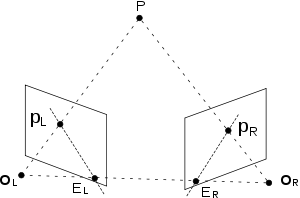
\includegraphics[height=5cm]{imagens/geometriaEpipolar.png}
		\caption{Triangulação utilizada na geomtria epipolar}
		\label{fotoGeometriaEpipolar}
	\end{figure}
	
		\subsection{Cinema 3D através de Estereoscopia}
		
		Em \cite{disneyRelatedWork} vê-se a sugestão de um complexo sistema motorizado de câmeras de vídeo com um ajuste automático de parâmetros de calibração para maior precisão na determinação de características tridimensionais obtidas através do sistema de câmeras estéreo proposto.
		
		Esta abordagem é efetiva para os autores dada a sua finalidade cinematográfica; e já que filmes em 3D são cada vez mais comuns nas salas de cinema em todo mundo, o investimento feito para obter a precisão que este trabalho alcança é facilmente compensado.
		
		Em um contexto mais amplo, que não suporta uma infra-estrutura complexa de uma filmagem dos estúdios de cinema internacionais ou demanda um dinamismo maior, o uso de um sistema motorizado de câmeras em sincronia é uma estratégia pouco eficiente, apesar da sua grande eficácia.
		
		\subsection{Um Abordagem Mais Simples da Estereoscopia}
		
		\cite{stereoRelatedWork} utiliza uma abordagem mais enxuta da reconstruçao 3D através de estereoscopia, sob a premissa de que as dimensões do objeto a ser reconstruído são conhecidas. Tal premissa, mesmo válida para o trabalho citado, reduz drasticamente o escopo da técnica sugerida.
		
		Usando um único par de imagens estereoscópicas estáticas e as dimensões do objeto estudado ainda é preciso efetuar alguns processos de normalização a ajuste algébrico para que condições de convergência, como o epipolo, possam ser obtidas. Tais empecilhos, inclusive, são decorrentes de uma análise do objeto em termos de coordenadas absolutas, o que é irrelevante para a análise de um objeto isolado cuja reconstrução não faz parte de um cenário igualmente importante.
		
		Assim, a reconstrução 3D de \cite{stereoRelatedWork} ainda não se adapta completamente ao objetivo deste trabalho.
		
	\section{Calibração de Câmera e Geometria Projetiva}
		\label{secaoEstadoDaArteCalibracao}
	
		Um conceito conhecido na computação gráfica é o de câmera virtual - um modelo matemático computacional que representa o funcionamento de um dispositivo de captura \cite{fundCompGraf}. A técnica de calibração de câmera consiste em estimar os parâmetros de uma câmera virtual capaz de produzir uma imagem. Uma vez que imagens são produzidas através de projeções, com o uso da geometria projetiva é possível haver dedução, sob certas hipóteses, de dados 3D após a análise de uma única imagem 2D.
		
		Em \cite{3DFromLineDrawings}, após um processo de obtenção dos parâmetros de uma câmera, é possível transformar polígonos pertencentes ao plano da imagem em polígonos equivalentes pertencentes a planos tridimensionais distintos do plano da imagem. Infortunadamente, esta referência não fora conhecida tão cedo quanto desejado, impedindo que este trabalho pudesse ter maior embasamento e robustez baseado em tal referência. No entanto, trabalhos parecidos sobre calibração de câmera para reconstrução 3D, que, estes sim, serviram como embasamento inicial, estão presentes em \cite{juizVirtual} e \cite{szenbergDoutorado}
\chapter{Materiais e Métodos}
	\label{materiaisEMetodos}

	Para a concretização deste trabalho, são necessários materiais tanto de ordem computacional, para processamento e implementação de software, tanto de ordem de dados, principalmente para teste das hipóteses encontradas, verificação de sucesso e embasamento teórico. 
	
	Os materiais em forma de dados devem consistir, basicamente, em imagens de objetos isolados e, de preferência, com elementos dispensáveis como plano de fundo e texturas padronizados e sistema ortogonal de coordenadas de referência, a fim de facilitar o processamento dos dados pelo computador e o funcionamento dos algoritmos desenvolvidos; foi conseguido um número suficiente, para o início do trabalho, de imagens que correspondiam a este padrão desejado através de repositórios \textit{on-line}. 
	
	A demanda por recursos computacionais de alta eficiência é baixa, portanto, pode-se, utilizar o computador pessoal do autor sem prejuízo de tempo; além disto, serão utlizadas ferramentas computacionais de terceiros, como bibliotecas de linguagens de programação e ambientes de edição de código-fonte, sob licença acadêmica gratuita, portanto, não acarretando em custos financeiros para a execução do trabalho.
	
	Tendo em vista o escopo bem definido e a um conjunto de materiais de aplicação estrito deste trabalho, foi buscado um método de desenvolvimento adequado à esta produção que, por não visar a solução de um problema de grande amplitude no universo da computação gráfica, pode ser dito como enxuto. A escolha considerada apropriada para tal cenário de trabalho é a metodologia Lean, também chamada de metodologia Enxuta.
	
\section{Recursos Computacionais}

	Não havendo grande volume de dados ou alta complexidade no processamento dos dados, será utilizado o computador pessoal textit{Notebook} Mobile Sim+ 6220 do autor do trabalho, com a seguinte configuração:
\begin{itemize}
	\item processador Intel\textregistered Core\textregistered i3 330M (2,13 GHz, 3MB Cache);
	\item memória RAM Kingston\textregistered PC3-8500 (4MB, DDR3);
	\item chipset gráfico Intel\textregistered HM55;
	\item sistema operacional Windows 7\textregistered.
\end{itemize}

	Para fins de construção de programas de computador e otimização do rendimento dos códigos-fontes em relação ao \textit{hardware} disponível, serão usadas as seguintes ferramentas computacionais:
\begin{itemize}
	\item Ambiente gráfico para programação em linguagem C\# Microsoft Visual Studio 2010 v4.5.50938 RTMRel\textregistered;
	\item Biblioteca de métodos algébricos em C\# ALGLIB Free Edition v3.8.2
	\item Software de visualização 3D Meshlab v1.3.3.
\end{itemize}

\section{Conjunto de Dados}

	Os dados utilizados como entrada nos algoritmos e programas desenvolvidos neste trabalho consistem em imagens digitais representando objetos apresentados no capítulo \ref{introducao}, o \textit{VW Beetle} de Sutherland (figura \ref{sutherlandVWDuplo}), o Bule de Leite de Newell (figura \ref{utahMilkjugDuplo}) e uma litografia digitalizada de Dürer (figura \ref{durerPerspectiva}). Todas as imagens utilizadas neste trabalho foram obtidas respeitando os direitos autorais e de reprodução.
	
	Quanto ao \textit{VW Beetle} de Sutherland, conseguiu-se obter uma imagem com sistemas ortogonais de coordenadas de referência graficamente evidentes (figura \ref{sutherlandVWDuplo3}), no entanto todas as imagens apresentavam-se em projeção em perspectiva, distorcendo as linhas do sistema de referência. Todas as imagens referentes a este objeto apresentavam regiões desprezíveis, como plano de fundo, facilmente diferenciáveis através de cor. Em formato `JPG', as imagens possuíam resolução de 72 dpi e 24 bits para intensidade de cor.

\begin{figure}[!htb]
	\centering
	\subfloat[\textit{VW Beetle} de Sutherland renderizado \cite{renderingSutherlandVW}]{
		\includegraphics[height=5cm]{imagens/SutherlandsVW-Skinned.jpg}
		\label{sutherlandVWDuplo1}
	}
	\quad
	\subfloat[\textit{VW Beetle} de Sutherland em \textit{wireframe} \cite{wireframeSutherlandVW}]{
		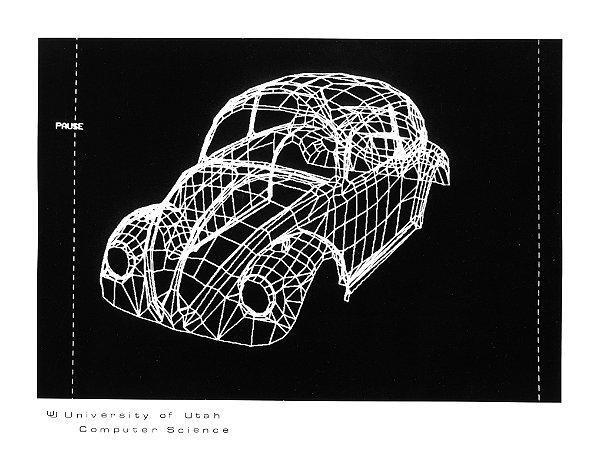
\includegraphics[height=5cm]{imagens/SutherlandsVW-Wireframe.jpg}
		\label{sutherlandVWDuplo2}
	}
	\quad
	\subfloat[\textit{VW Beetle} de Sutherland com referências \cite{jalopnik}]{
		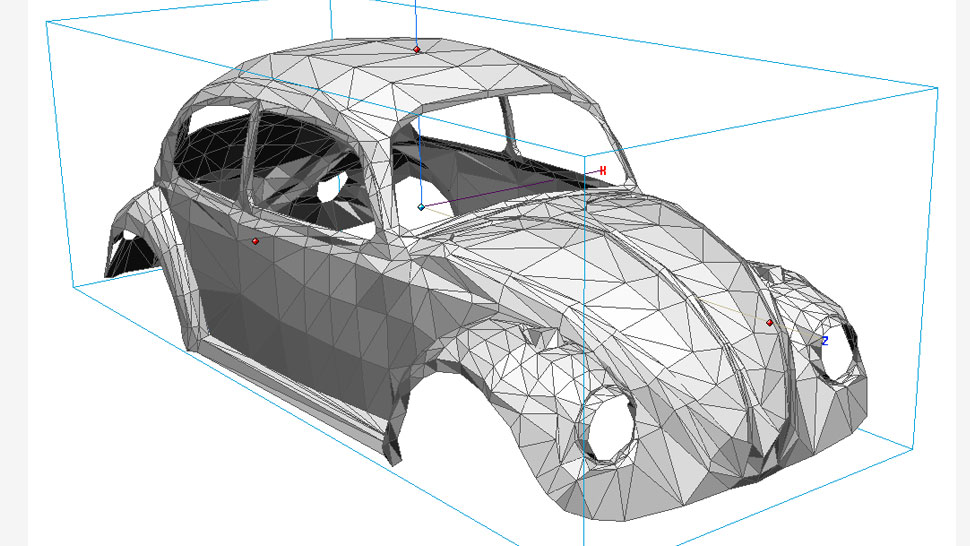
\includegraphics[height=5cm]{imagens/SutherlandsVW-Skinned-Referenced.jpg}
		\label{sutherlandVWDuplo3}
	}
	\caption{O \textit{VW Beetle} de Sutherland}
	\label{sutherlandVWDuplo}
\end{figure}
	
	As imagens do Bule de Leite de Newell, por este ser um objeto sem registro oficial dos seus dados, são menos elaboradas, com o sistema de coordenadas de referência mais nebuloso, mas, afortunadamente, apresentando projeção paralela isométrica. Tais imagens são em branco e preto, em formato `PNG' com 32 bits para intensidade de cor e resolução de 95 dpi.

\begin{figure}[!htb]
	\centering
	\subfloat[Bule de Leite de Newell convencional \cite{newellResearch}]{
		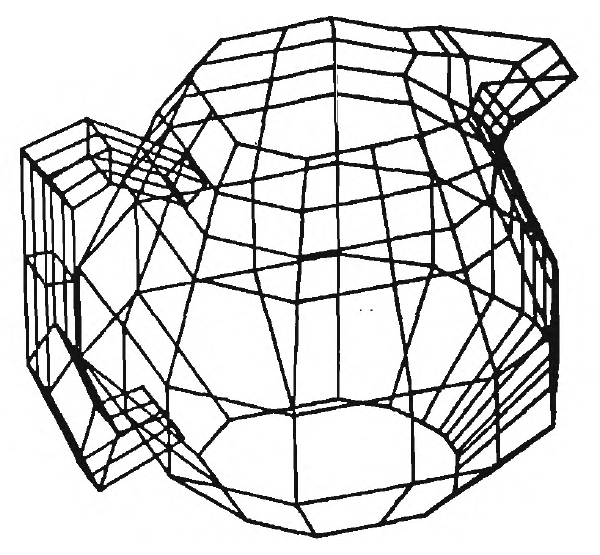
\includegraphics[height=5cm]{imagens/Milkjug-Wireframe-1.png}
		\label{utahMilkjugDuplo1}
	}
	\quad
	\subfloat[Bule de Leite de Newell suavizado \cite{newellResearch}]{
		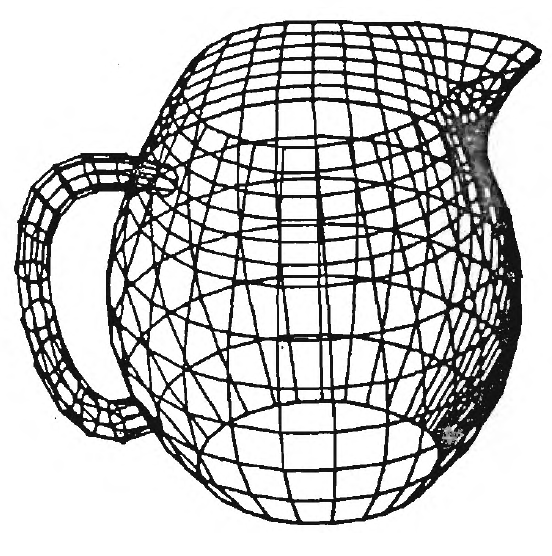
\includegraphics[height=5cm]{imagens/Milkjug-Wireframe-2.png}
		\label{utahMilkjugDuplo2}
	}
	\caption{O Bule de Leite de Newell}
	\label{utahMilkjugDuplo}
\end{figure}

	A litografia de Dürer, digitalizada e disponibilizada por terceiros, possui um sistema de referências evidente e, como se pode prever, está representada através da projeção em perspectiva. Em formato `JPG' com 96 dpi de resolução e 24 bits de profundidade de cor.
	
\begin{figure}[!htb]
	\centering
	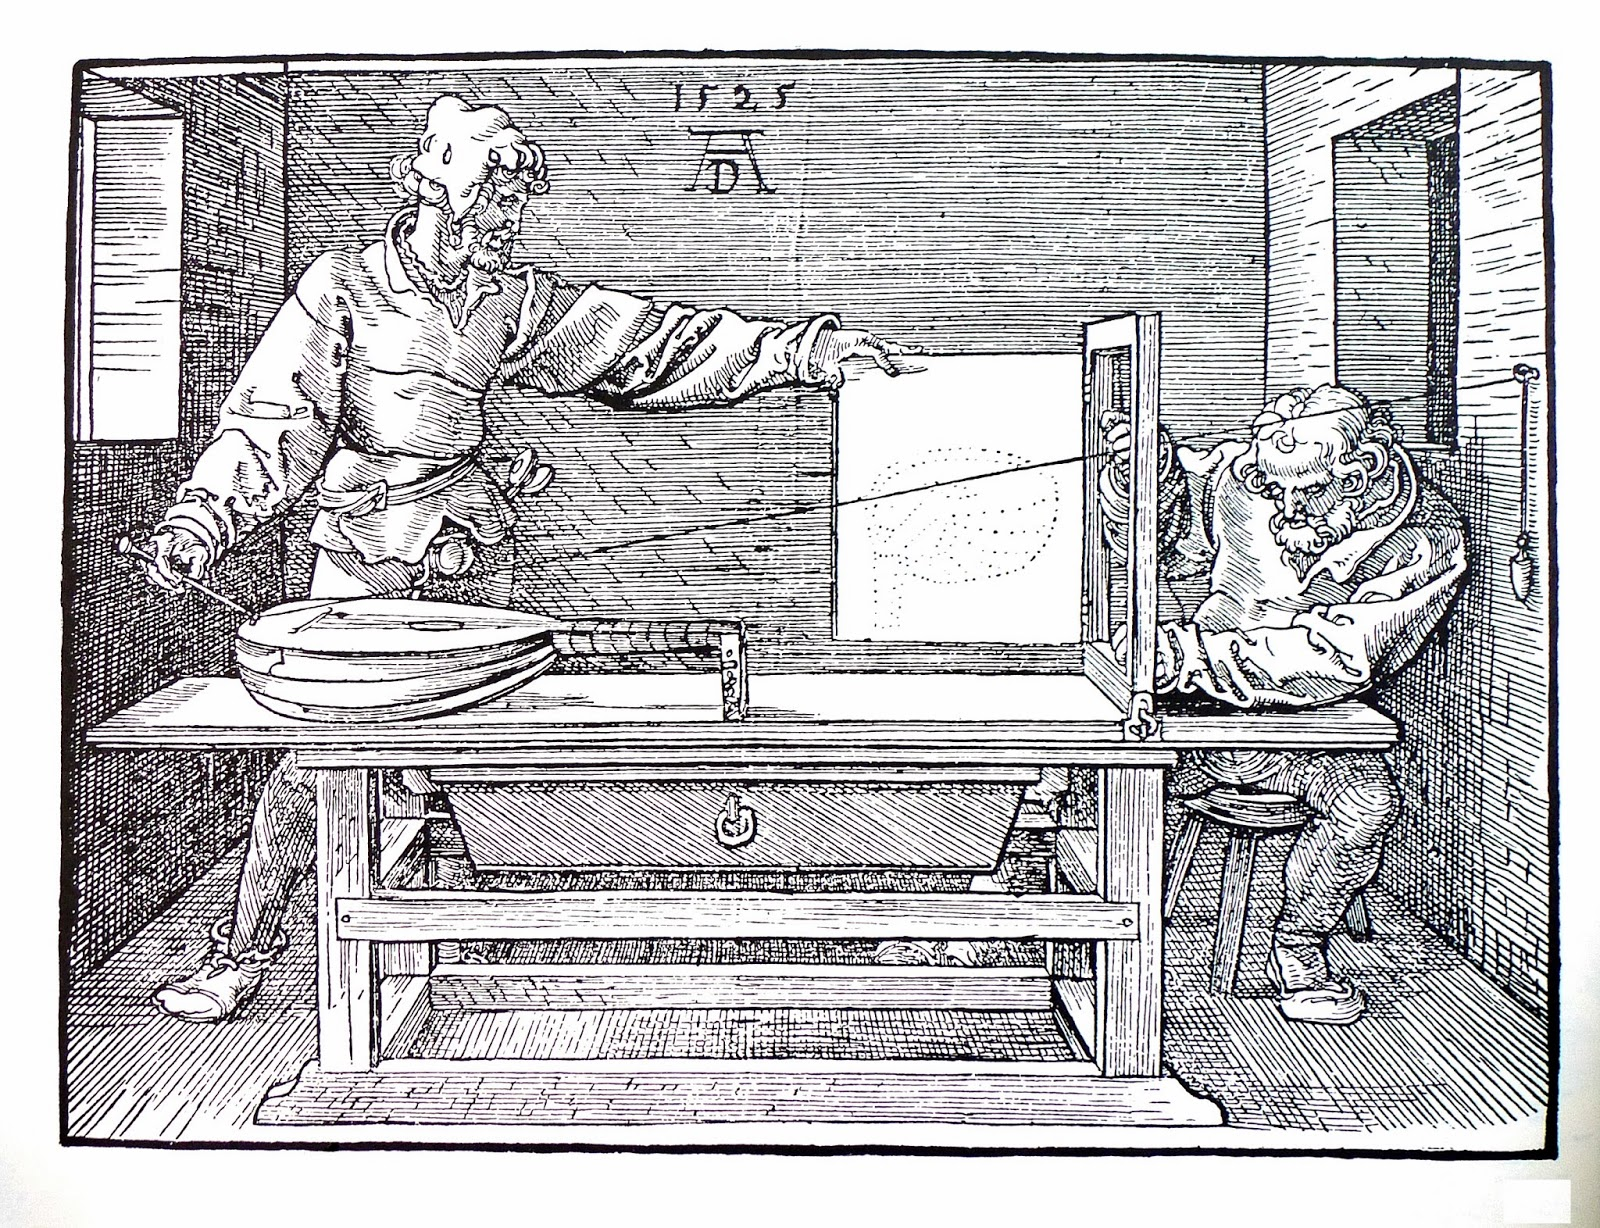
\includegraphics[height=7cm]{imagens/durer.jpg}
	\caption{A litografia de Dürer \cite{durerSite}}
	\label{durerPerspectiva}
\end{figure}
	
\section{Aferição da corretude}

	Como o objetivo deste trabalho é reconstruir objetos cujas informações tridimensionais são inexistentes, é impossível se fazer uma validação direta dos resultados obtidos, isto é, não há como comparar os modelos tridimensionais obtidos neste trabalho com um modelo paramétrico dos mesmos objetos estudados.

	De tal forma, a corretude dos modelos obtidos será obtida de forma implícita, através da validação da técnica de reconstrução deste trabalho. Utilizando cenas específicas confeccionadas pelo autor (figuras \ref{cenasValidacao}), nas quais os elementos a serem reconstruídos têm suas informações catalogadas, será estimado um erro geométrico $E$ (fórmula \ref{formulaErroGeometricoMedio}) entre os pontos de coordenadas conhecidos dos modelos (P) e os pontos de coordenadas obtidos pela técnica desenvolvida neste trabalho (P'). 
	
\begin{equation}
	\label{formulaErroGeometricoMedio}
	E = \sqrt{(x_{P_i} - x_{P'_i})^2 + (y_{P_i} - y_{P'_i})^2 + (z_{P_i} - z_{P'_i})^2} 
\end{equation}
	
\begin{figure}[!htb]
	\centering
	\subfloat[Cena específica 1, um cubo unitário]{
		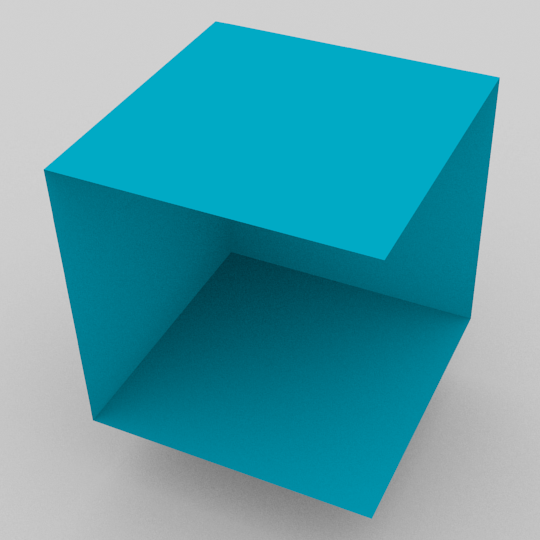
\includegraphics[height=4cm]{imagens/cenaTeste1.png}
		\label{cenaValidacao1}
	}
	\quad
	\subfloat[Cena específica 2, uma pirâmide regular equilátera unitária]{
		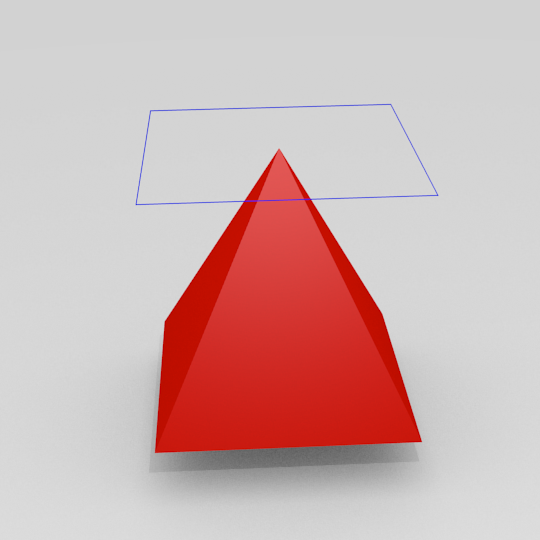
\includegraphics[height=4cm]{imagens/cenaTeste2.png}
		\label{cenaValidacao2}
	}
	\quad
	\subfloat[Cena específica 3, um cubo de dimensão $0.5$]{
		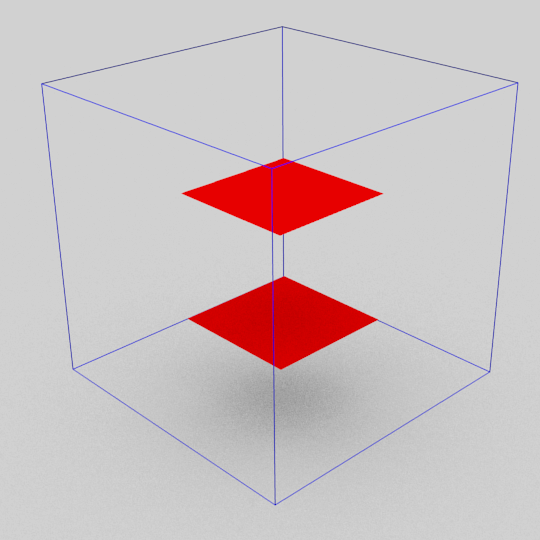
\includegraphics[height=4cm]{imagens/cenaTeste3.png}
		\label{cenaValidacao3}
	}
	\caption{Cenas para validação da técnica de reconstrução}
	\label{cenasValidacao}
\end{figure}

	Com a cena de validação 1 (figura \ref{cenaValidacao1}) deseja-se a reconstrução dos vértices de um hexaedro de dimensão unitária; com a cena de validação 2 (figura \ref{cenaValidacao2}) almejam-se os vértices de uma pirâmide regular equilátera de dimensão unitária; por fim, com a cena de validação 3, buscam-se os vértices de um cubo de dimensão $0.5$. 
	
	Nas cenas de validação há um plano abaixo do objeto descrito anteriormente, este não será reconstruído, servindo apenas como aparato visual na imagem da cena. Na cena de validação 1 (figura \ref{cenaValidacao1}), um cubo (hexaedro) teve duas de suas faces removidas, a fim facilitar a demarcação de pontos de referência, originando a figura vista. No caso da figura \ref{cenaValidacao2}, há, ainda, um quadrado de cor azul paralelo ao plano da base da pirâmide; tal quadrado é um auxílio, inserido pelo autor, para a demarcação dos pontos de referência e também será desconsiderado como objeto em reconstrução. A figura \ref{cenaValidacao3}, por sua vez, apresenta as arestas (em azul) de um cubo, estas são um auxílio para a demarcação de referências; note que neste cena também foram removidas faces do cubo para facilitar demarcações.

	Todas as imagens das cenas de validação têm resolução de 72 dpi.
\chapter{Fundamentação Teórica}
	\label{capituloReferencialTeorico}
	Neste trabalho de conclusão de curso, são usados alguns conceitos e técnicas da computação gráfica de forma adaptada ao objetivo proposto. Nas próximas seções são explicados os conceitos utilizados e suas respectivas aplicações no trabalho desenvolvido.
	
	\section{Projeções}
		\label{secaoProjecoes}
		
		Inicialmente, projeções são representações de objetos sob as restrições de um determinado ambiente. Em geometria analítica usam-se projeções para a descrição de vetores (as componentes do vetor são as projeções deste em cada uma das bases do sistema ordenado); no cotidiano, sombras geradas pelo nosso corpo no chão, por exemplo, é um caso específico de projeção (representação) do nosso corpo (objeto) na superfície plana do chão (ambiente) \cite{archiGeoBook}.
		
		Em computação gráfica, as projeções servem para representar objetos tridimensionais em dispositivos de visualização bidimensionais. Dependendo da utilização da visualização, diferentes formas de projetar o objeto tridimensional podem ser usadas \cite{archiGeoBook}; as duas principais são a projeção paralela e a projeção cônica.
		
		Independente do tipo de projeção, com apenas uma imagem não se pode estabelecer uma relação unívoca entre pontos no plano de projeção e pontos no espaço \cite{foto3D}. No entanto, relações de isometria (seção \ref{subsecaoProjecaoParalela}) ou proporcionalidade (seção \ref{subsecaoProjecaoConica}) podem incutir restrições aos pontos no espaço de forma a reduzir tal multiplicidade.
		
		\subsection{Projeção Paralela}
			\label{subsecaoProjecaoParalela}
			A projeção gráfica pode ser feita através de linhas paralelas entre si que ligam pontos do objeto ao plano de projeção (figura \ref{imagemProjecaoParalela}); esta projeção é chamada de projeção paralela \cite{archiGeoBook}. Neste caso, são mantidas as proporções entre as dimensões do objeto estudado (isometria) \cite{fundCompGraf}.
		
		\begin{figure}[!htb]
			\centering
			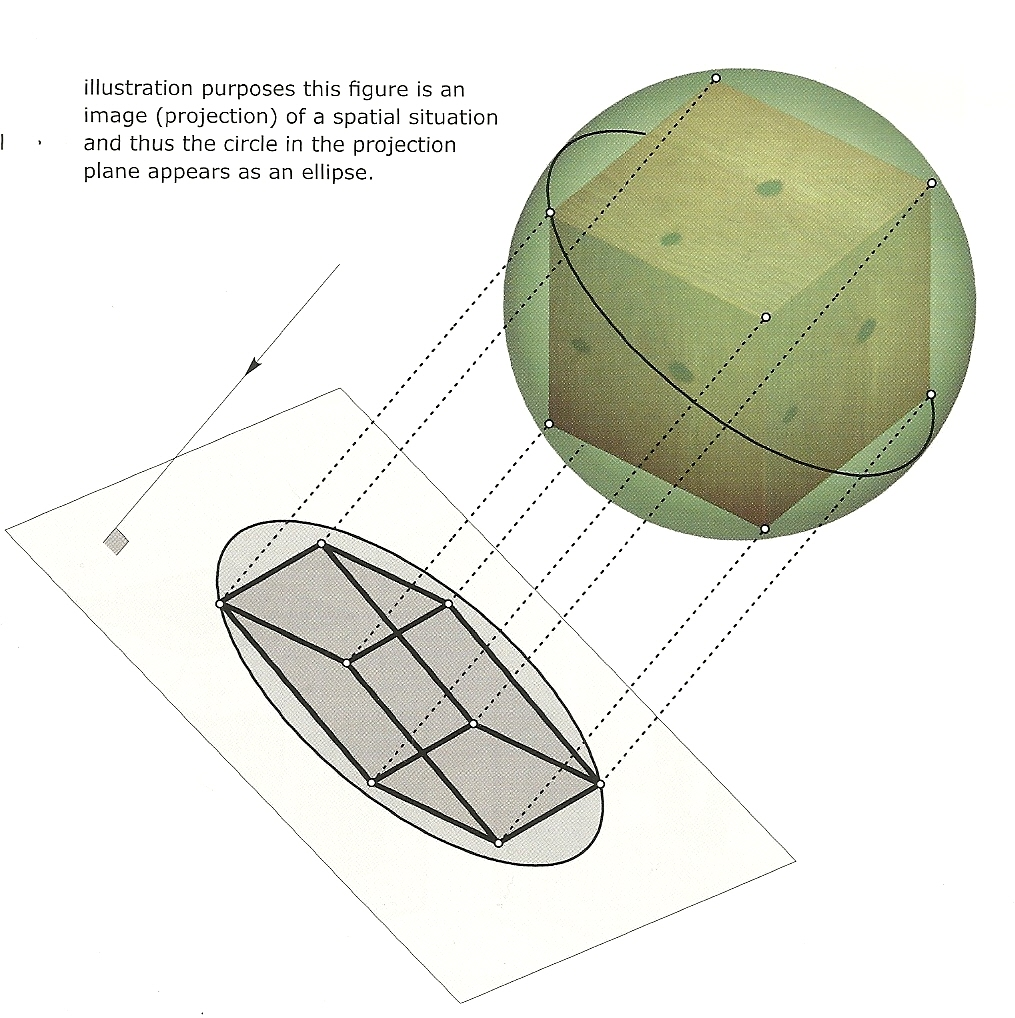
\includegraphics[height=5cm]{imagens/projecaoParalela.jpg}
			\caption{Projeção paralela em \cite{archiGeoBook}}
			\label{imagemProjecaoParalela}
		\end{figure}
		
			A isometria é uma característica interessante deste tipo de projeção pois todas as condições de paralelismo são mantidas.
			
			A transformação de um ponto 3D $P = (X_P, Y_P, Z_P)$ em um ponto 2D $P'$ sob a projeção paralela é dada pela equação \ref{formulaProjecaoParalela}, em coordenadas baseadas no Sistema de Coordenadas da Câmera \cite{foto3D}. Como pode-se notar, a projeção de $P$ independe da sua distância - $Z_P$ - ao plano de projeção e isto causa a multiplicidade projetiva.
			
			\begin{equation}
				\label{formulaProjecaoParalela}
				P' = (X_P, Y_P)
			\end{equation}
			
		\subsection{Projeção Cônica}
			\label{subsecaoProjecaoConica}
			Com o intuito de representar um objeto de forma similar à realidade, é aplicada a projeção cônica (ou perspectiva) \cite{archiGeoBook}. Tal projeção provoca uma deformação linear (equação \ref{formulaProjecaoConica}), proporcional à distância $Z_P$ ao plano de projeção, na posição planar do ponto $P = (X_P, Y_P, Z_P)$, que também está expresso em coordenadas do Sistema de Coordenadas da Câmera \cite{foto3D}. Isto se dá pois a projeção $P'$ de $P$ é a interseção da reta que une o ponto 3D $e$ ao ponto $P$ (figura \ref{imagemProjecaoConica}), sendo $e$ o centro de projeção, que funciona de forma análoga ao olho de um observador humano \cite{archiGeoBook}.
			
			\begin{equation}
				\label{formulaProjecaoConica}
				P' = \left (\frac{X_P}{Z_P}, \frac{Y_P}{Z_P}\right )
			\end{equation}
			
			\begin{figure}[!htb]
				\centering
				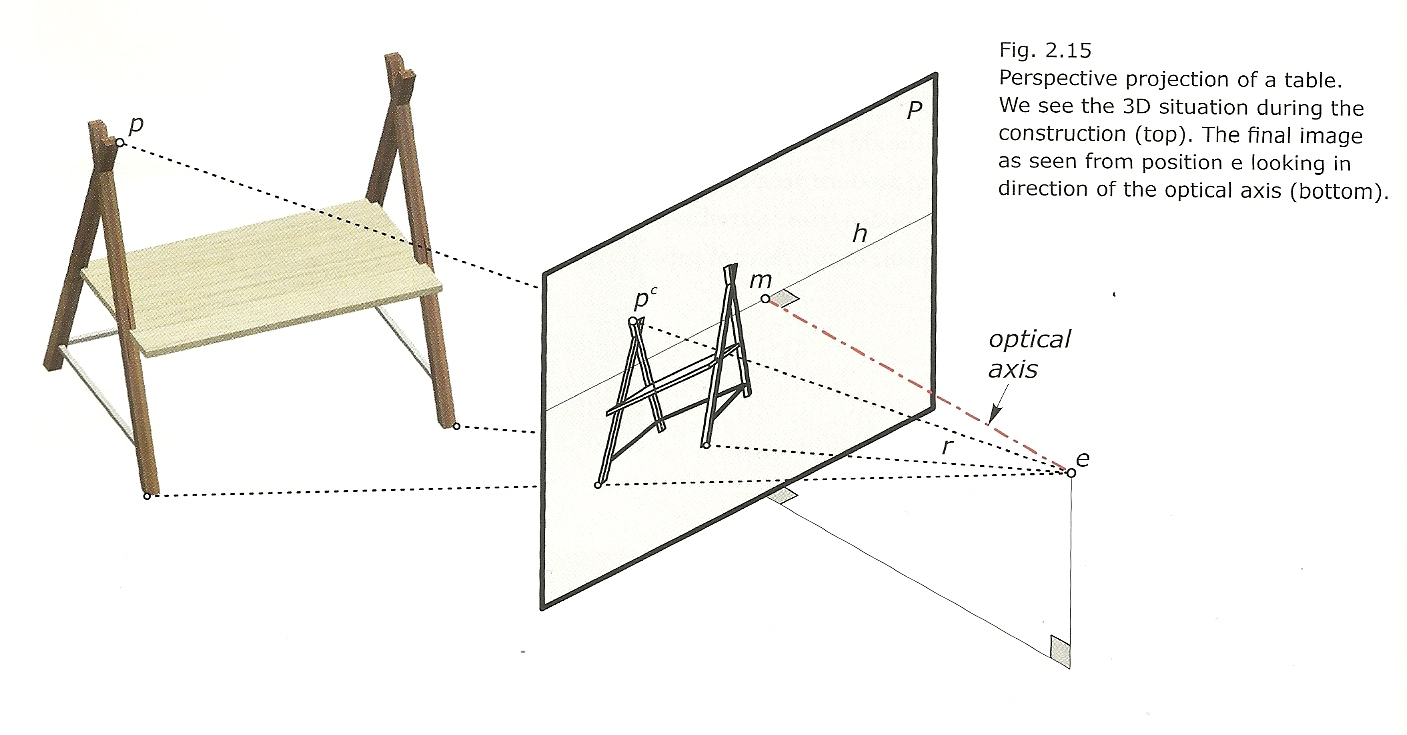
\includegraphics[height=5cm]{imagens/projecaoConica.jpg}
				\caption{Projeção cônica em \cite{archiGeoBook}}
				\label{imagemProjecaoConica}
			\end{figure}
			
			A deformação provocada pela projeção cônica impossibilita a existência da isometria, no entanto, o processo de calibração de câmera virtual (seções \ref{secaoCamera} e \ref{secaoCalibracao}) possibilita relações entre pontos 2D e 3D \cite{juizVirtual}.
	
	\section{Câmera Virtual}
		\label{secaoCamera}
	
		A operação básica de uma câmera virtual é a projeção \cite{fundCompGraf}. A fim de sintetizar uma imagem de um objeto digital com três dimensões, programas de visualização 3D implementam um modelo matemático que utiliza as técnicas discutidas anteriormente (seção \ref{secaoProjecoes}) para a transformação de 3D para 2D.
		
		Neste trabalho optou-se por desenvolver um modelo de câmera que projeta apenas em perspectiva, dada a ausência, inicialmente, de bibliografia sobre modelos de câmeras de projeção paralela. No entanto, na seção \ref{secaoEstadoDaArteCalibracao} é exposta uma possibilidade de retificação desta limitação.
		
		Para um modelo altamente fiel à câmera real, devem ser feitas correções acerca de distorções de lentes \cite{animation} além de que uma câmera digital real, em termos geométricos, precisa converter as coordenadas de um objeto sob um sistema de referências global para um sistema de coordenadas em \textit{pixels} passando por um sistema de coordenadas de câmera e de imagem, processos chamados de Transformações de Câmera \cite{foto3D}. Para este trabalho, não há distorção de lentes nas imagens (uma vez que são artificiais).
		
		Em \cite{foto3D} é descrita cada transformação entre cada sistema de coordenadas. No entanto, neste trabalho todas as transformações de câmera foram agrupadas, como em \cite{juizVirtual} e \cite{fundCompGraf}, uma vez que apenas interessa a transformação final e não os parâmetros explícitos da câmera. Assim, o modelo final de câmera $C$ utilizado foi o apresentado na equação \ref{formulaCamera}.
		
		\begin{equation}
			C = \begin{pmatrix}
						q_{1,1} & q_{1,2} & q_{1,3} & q_{1,4} \\
						q_{2,1} & q_{2,2} & q_{2,3} & q_{2,4} \\
						q_{3,1} & q_{3,2} & q_{3,3} & q_{3,4}
					\end{pmatrix}
			\label{formulaCamera}
		\end{equation}
		
		De forma que, aplicando $C$ a um ponto 3D, em coordenadas homogêneas \cite{fundCompGraf2} sob o Sistema de Coordenadas do Mundo \cite{foto3D}, obter-se-á diretamente o respectivo ponto 2D em termos de \textit{pixel} na imagem.
	
	\section{Calibração de câmera}
		\label{secaoCalibracao}
	
		Costumeiramente, o modelo de câmera virtual é construído a partir dos parâmetros (intrínsecos e extrínsecos) \cite{fundCompGraf} da câmera; pode-se dizer que esta é a forma direta de especificação da câmera. 
		
		Neste trabalho, um dos empecilhos era o desconhecimento destes atributos da câmera, mas sem tal conhecimento não há como construir a transformação \ref{formulaCamera}. No entanto, com uma correspondência previamente conhecida entre pontos da imagem e pontos 3D, o modelo da câmera pode ser estimado através de um processo chamado de Calibração de Câmera (costuma-se chamar, também, de \textit{Resectioning}, já que calibração pode envolver, ainda, ajuste cromático). \cite{juizVirtual}, \cite{szenbergDoutorado} e \cite{lectureCameraCalibration} aplicam apenas a calibração geométrica e usam o termo "Calibração".
		
		Como dito na seção \ref{secaoCamera}, a aplicação do modelo de câmera em pontos 3D $P = (X, Y, Z)$ leva a pontos 2D $P' = (u, v)$ da imagem; de forma que, segundo \cite{juizVirtual}, têm-se para cada correspondência de pontos 3D com 2D as equações \ref{formulaSistemaSimples1} e \ref{formulaSistemaSimples2}.
	
	\begin{equation}
		\label{formulaSistemaSimples1}
		u = \left(\frac{q_{1,1} . X + q_{1,2} . Y + q_{1,3} . Z + q_{1,4}}{q_{3,1} . X + q_{3,2} . Y + q_{3,3} . Z + q_{3,4}} \right)
	\end{equation}
	
	\begin{equation}
		\label{formulaSistemaSimples2}
		v = \left(\frac{q_{2,1} . X + q_{2,2} . Y + q_{2,3} . Z + q_{2,4}}{q_{3,1} . X + q_{3,2} . Y + q_{3,3} . Z + q_{3,4}} \right) 
	\end{equation}
	
	Como a matriz $C$ da câmera (equação \ref{formulaCamera}) tem 12 graus de liberdade, são necessários, no mínimo, 6 correspondências, com pontos 3D linearmente independentes, para que se monte um sistema dado por \ref{formulaSistemaMontado} possível de ser resolvido \cite{lectureCameraCalibration}.
	
	\begin{equation}
		\label{formulaSistemaMontado}
		\setcounter{MaxMatrixCols}{20}
		\begin{pmatrix}
			X_{1} & Y_{1} & Z_{1} & 1 & 0 & 0 & 0 & 0 & -u_{1}X_{1} & -u_{1}Y_{1} & -u_{1}Z_{1} & -u_{1} \\
			0 & 0 & 0 & 0 & X_{1} & Y_{1} & Z_{1} & 1 & -v_{1}X_{1} & -v_{1}Y_{1} & -v_{1}Z_{1} & -v_{1} \\
			\vdots & \vdots & \vdots & \vdots & \vdots & \vdots & \vdots & \vdots & \vdots & \vdots & \vdots & \vdots \\
			X_{n} & Y_{n} & Z_{n} & 1 & 0 & 0 & 0 & 0 & -u_{n}X_{n} & -u_{n}Y_{n} & -u_{n}Z_{n} & -u_{n} \\
			0 & 0 & 0 & 0 & X_{n} & Y_{n} & Z_{n} & 1 & -v_{n}X_{n} & -v_{n}Y_{n} & -v_{n}Z_{n} & -v_{n}	
		\end{pmatrix}
		.
		\begin{pmatrix}
			q_{1,1} \\
			q_{1,2} \\
			q_{1,3} \\
			q_{1,4} \\
			q_{2,1} \\
			q_{2,2} \\
			q_{2,3} \\
			q_{2,4} \\
			q_{3,1} \\
			q_{3,2} \\
			q_{3,3} \\
			q_{3,4} \\
		\end{pmatrix}
		=
		\begin{pmatrix}
			0 \\
			0 \\
			0 \\
			0 \\
			0 \\
			0 \\
			0 \\
			0 \\
			0 \\
			0 \\
			0 \\
			0 \\
		\end{pmatrix}
	\end{equation}
	
	O problema \ref{formulaSistemaMontado} é, costumeiramente, impreciso devido a erros na coleta dos valores dos pontos, neste trabalho, isto acontece devido a imprecisão do \textit{mouse} ao demarcar \textit{pixels} (vide capítulo \ref{capituloReconstrucao}). Assim, usa-se um aproximação pelo método dos mínimos quadrados.
	
	Pelo método dos mínimos quadrados, busca-se o melhor valor para a matriz $C$ solucionar o sistema \ref{formulaSistemaMontado} dada uma restrição que impeça de se chegar à solução trivial ($C = 0$). Em \cite{juizVirtual} buscou-se uma restrição linear. No entanto, por trabalhar em coordenadas homogêneas, $C$ é independente de escala ($\lambda C \cong C$), podendo-se adotar a restrição $|C| = 1$ \cite{lectureCameraCalibration}.
	
	Por conseguinte, este é um problema de minimização solucionável por multiplicadores de Lagrange, onde se chega à expressão \ref{formulaMinimizacaoLagrange}. Observa-se que a solução $Q$ é um autovetor de $A^TA$ e, para a maior minimização, $Q$ deve ser o autovetor gerado pelo menor autovalor de $A^TA$. \cite{lectureLeastSquares}
	
	\begin{equation}
		\label{formulaMinimizacaoLagrange}
		A^TA . Q = \lambda . Q
	\end{equation}
	
	Por fim, a organização dos valores de $Q$ na forma de $C$ completa o processo de calibração da câmera; o que permite a busca de pontos 3D correspondentes a pontos 2D da imagem (capítulo \ref{capituloReconstrucao}).

\chapter{A Técnica de Reconstrução}
	\label{capituloReconstrucao}

	Em posse do referencial teórico descrito no capítulo \ref{capituloReferencialTeorico}, a reconstrução de um objeto se deu através da indicação de pontos de interesse na imagem e da implementação de hipóteses de restrição geométrica, baseadas na transformação de câmera encontrada, a fim de eliminar a multiplicidade inerente às correspondência projetiva (seção \ref{secaoProjecoes}).

	Inicialmente, é necessário descobrir qual matriz de transformação projetiva é capaz de gerar tal imagem do objeto. Tal conhecimento permite conhecer a posição 2D, no sistema de coordenadas da imagem e sob seu mesmo ponto de vista, que corresponde a qualquer ponto 3D do espaço. Como discutido na seção \ref{secaoCalibracao}, 6 correspondências entre pontos 2D e 3D, conhecidas previamente, são o bastante para fornecer uma aproximação da transformação desejada; no entanto, neste trabalho são usadas 8 correspondências, obrigatoriamente entre os pontos 3D $P = \{(x, y, z) | 0 \leq x, y, z \leq 1\}$.
	
	Tal restrição tem o intuito de simplificar a entrada de dados do usuário no aplicativo de reconstrução (seção \ref{appReconstrucao}) e garantir a satisfação da condição de independência linear para a boa execução do método de calibração (seção \ref{secaoCalibracao}).
	
	Após o processo de calibração já é possível descobrir se um ponto 3D tem sua projeção coincidente com um ponto de interesse na imagem, assim, por força-bruta, infere-se a posição 3D no espaço dos pontos de interesse 2D da imagem. 
	
	No entanto, resta, ainda, o problema da multiplicidade de pontos; sabendo-se que isto se dá devido a formação da imagem ser feita através da interseção entre a reta de projeção (reta que liga o ponto 3D retratado ao centro de projeção da câmera) e o plano de projeção (figura \ref{imagemProjecaoConica}).
	
	Analisando o cenário que contém o objeto, nota-se que a reta de projeção contém vários pontos 3D, mas cada um destes tem um valor exclusivo da coordenada $Z$ (figura \ref{imagemUnicoPontoPorPlano}); isto é provado pela geometria analítica, uma vez que a interseção entre uma reta (a reta de projeção, no caso) e um plano (no caso, um plano $Z = k$, com um $k$ qualquer) é um ponto.
	
	\begin{figure}[!htb]
		\centering
		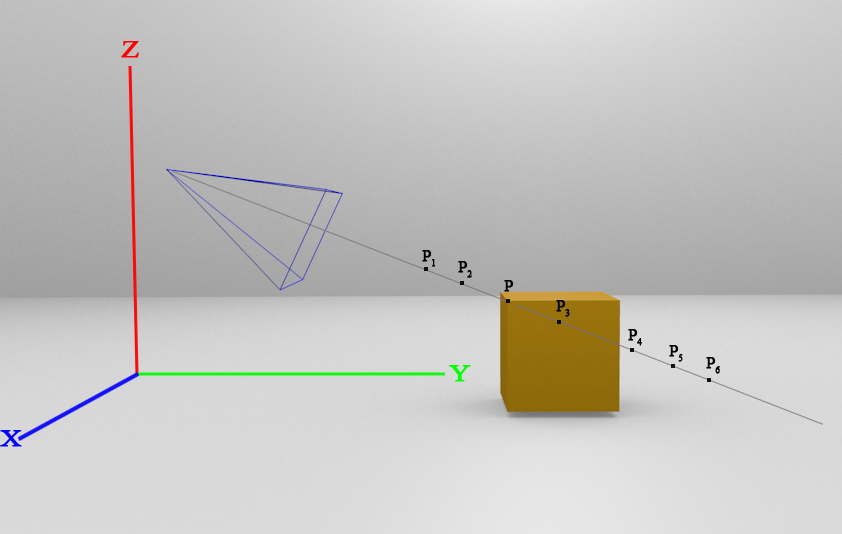
\includegraphics[height=6cm]{imagens/cenaExemploUnicoPontoPorPlano.png}
		\caption{Os pontos $P_i$ pertencem à reta de projeção de $P$, mas suas coordenadas Z são diferentes da coordenada Z do ponto $P$}
		\label{imagemUnicoPontoPorPlano}
	\end{figure}
	
	Se, ao indicar o ponto de interesse, fosse fornecido o seu valor da coordenada Z, determinar seu correspondente 3D no espaço seria uma tarefa banal com uma demanda exaustiva por dados do usuário. Em viés, sem informações além da transformação projetiva e coordenadas 2D do ponto de interesse não há formas de determinar sua coordenada Z no espaço \cite{foto3D}.
	
	No entanto, devido ao apelo visual da imagem, é fácil determinar se um ponto da imagem tem seu correspondente 3D com coordenada Z igual, ou aceitavelmente igual, à coordenada Z do correspondente 3D de outros pontos da imagem (figura \ref{imagemPontosMesmoPlano}). De forma que, ao fornecer os pontos de interesse para a reconstrução, indicar quais pontos de interesse da imagem têm seu correspondente 3D em uma mesma coordenada Z é simples e provê subterfúgios para a eliminação da multiplicidade projetiva.
	
	Neste trabalho, para cada grupamento é atribuído um identificador numérico inteiro, onde, quanto menor o identificador, menor o valor da coordenada Z do grupamento.
	
	\begin{figure}[!htb]
		\centering
		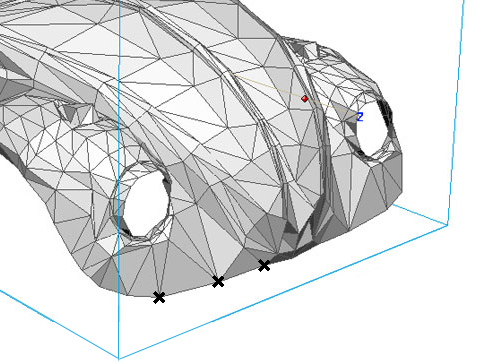
\includegraphics[height=5cm]{imagens/pontosMesmoPlano.png}
		\caption{É perceptível que os pontos demarcados com um "X" têm a mesma coordenada Z no espaço}
		\label{imagemPontosMesmoPlano}
	\end{figure}
	
	Assim, de posse de um grupamento de pontos da imagem com mesma coordenada Z, iterativamente, são descartados valores para a coordenada Z do grupamento que, pela transformação projetiva encontrada para a imagem, não possui um ponto possível de ser o correspondente 3D de algum dos pontos de interesse do grupamento em questão.
	
	Tal eliminação de multiplicidade por interseção é eficaz dado o seu embasamento geométrico citado anteriormente. No entanto, assim como no estabelecimento das correspondências (seção \ref{secaoCalibracao}), há imprecisão na demarcação dos pontos de interesse na imagem. Então, é compreensível que seja adotada uma tolerância projetiva. A tolerância projetiva diz respeito a quão longe do ponto demarcado como interessante à reconstrução um ponto 3D ainda pode projetar para ser considerado como correspondente a este; tolerâncias grandes levam à imprecisão de reconstrução, ao passo que tolerâncias pequenas levam à dificuldade em achar correspondentes. O valor da tolerância projetiva é definido pelo usuário no momento da reconstrução. 
	
	Tal tolerância pode causar a não convergência do algoritmo de eliminação de coordenadas Z por interseção para um único valor; neste caso, o valor da coordenada Z adotado é dado por um critério de convergência arbitrário. Neste trabalho foram usados os critérios:
	\begin{itemize}
		\item Adotar o valor mais próximo ao valor anteriormente definido (começando do zero); ou
		\item adotar o valor mais próximo à média dos valores possíveis dada a eliminação por intersecção.
	\end{itemize}
	
	Ainda em consequência da tolerância projetiva, um número finito de pontos com a mesma coordenada Z projetam próximo o suficiente do ponto de interesse. Assim, como correspondente 3D definitivo do ponto de interesse em questão é adotado o baricentro destes pontos adicionais.
	
	Não obstante, é necessário que se determine um espaço finito de busca destes correspondentes 3D, já que há pontos 3D que projetam em um ponto de interesse em infinitas posições do espaço. Para limitar a busca, então, são usados os mesmo pontos 3D aplicados na correspondência para calibração, isto é, os pontos $P = \{(x, y, z) | 0 \leq x, y, z \leq 1\}$. Como resultado, os pontos 3D reconstruídos terão suas coordenadas entre 0 e 1.
	
	Dentro do espaço de busca um quesito ainda importante é a distância ente dois valores consecutivos de uma coordenada (i.e. incremento) durante a iteração de busca. Incrementos menores levam à uma maior precisão da reconstrução, enquanto incrementos maiores tornam o algoritmo mais ágil. O valor do incremento é definido no início da reconstrução.
	
	Em suma, é importante ressaltar que esta técnica reconstrói apenas pontos 3D, arestas e planos podem ser adicionados à nuvem de pontos encontrada em um processo de pós-tratamento.
	
	
\chapter{Os Softwares}
	\label{capituloSoftwares}

	Ao decorrer deste trabalho, fora o software que implementa a técnica de reconstrução descrita nesta monografia, foi sendo necessário que técnicas adjuntas à estudada aqui também fossem implementadas em softwares a fim de facilitar comprovações de resultados e automatizações de tarefas auxiliares ao projeto; além de agregar determinada riqueza de esforço e de ferramentas a este trabalho de conclusão de curso.
	
	A seguir são apresentados os exemplos mais representativos dos softwares desenvolvidos ao longo do projeto.
	
	\section{Aplicativo de detecção de retas}
		\label{appDeteccaoRetas}
		Tanto para auxiliar na detecção automática dos segmentos de reta do sistema de coordenadas de referência quanto dos pontos (interseção de segmentos de reta) de interesse à reconstrução. Foi desenvolvido um aplicativo para a obtenção de parâmetros analíticos de retas apresentadas em uma região de uma imagem digital.
		
		As linhas inferidas como interessantes, por serem representadas através da rasterização - processo de conversão da representação vetorial para a matricial \cite{compGrafTeoPrat} - precisaram sofrer um processo de regressão linear a fim de se obter uma aproximação dos parâmetros geométricos analíticos de sua formação. A regressão linear executada para a obtenção dos coeficientes angular e linear das retas de interesse se deu através do método dos mínimos quadrados.
	
	O Métodos dos Mínimos Quadrados é uma técnica de regressão linear que busca ajustar corretamente coeficientes de uma curva algébrica de forma que estes minimizem o somatório do quadrado da diferença entre os valores dos dados reais e os valores estimados, minimizando o erro de aproximação.
	
	Com uma interface apropriada, pôde-se carregar uma imagem e, através da demarcação manual de uma região de interesse na mesma (demarcada por um retângulo vermelho), pontos da possível linha foram detectados pela sua cor preta e submetidos ao método dos mínimos quadrados (figura \ref{figMinQuadInterface}).
	
	Após a aproximação são exibidos, na parte superior da janela, os coeficientes encontrados e é plotada, sobre a imagem, a reta encontrada.
	
	\begin{figure}[!htb]
		\centering
		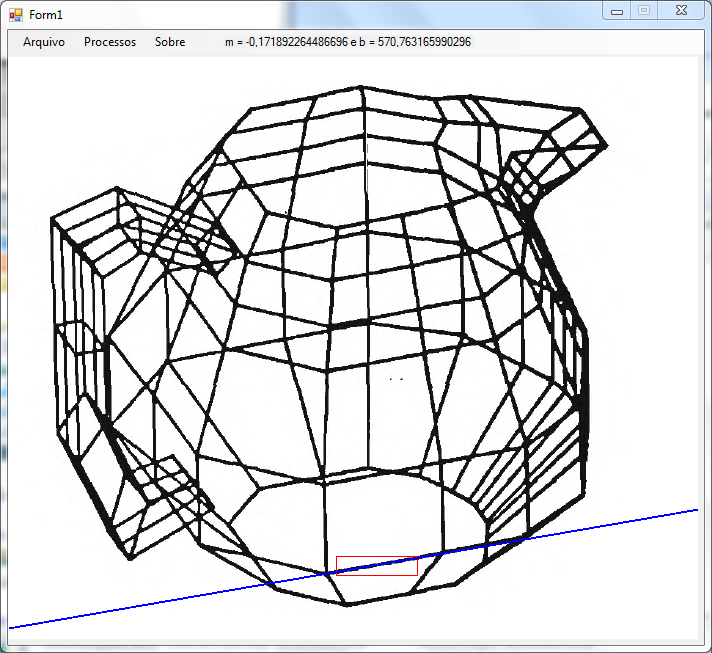
\includegraphics[height=6cm]{imagens/printAppMinimosQuadrados.png}
		\caption{O programa de regressão de rasterização com uma aproximação de exemplo}
		\label{figMinQuadInterface}
	\end{figure}

	Posteriormente, os coeficientes encontrados foram submetidos ao programa Microsoft Mathematics\textregistered  comprovando que os valores encontrados são coerentes (figura \ref{mathematics}). Note que, como o sentido de orientação dos pontos da imagem (de cima para baixo) é inverso ao do plano cartesiano (de baixo para cima) o aspecto da reta em relação ao aspecto da linha é invertido.
	
	\begin{figure}[!htb]
		\centering
		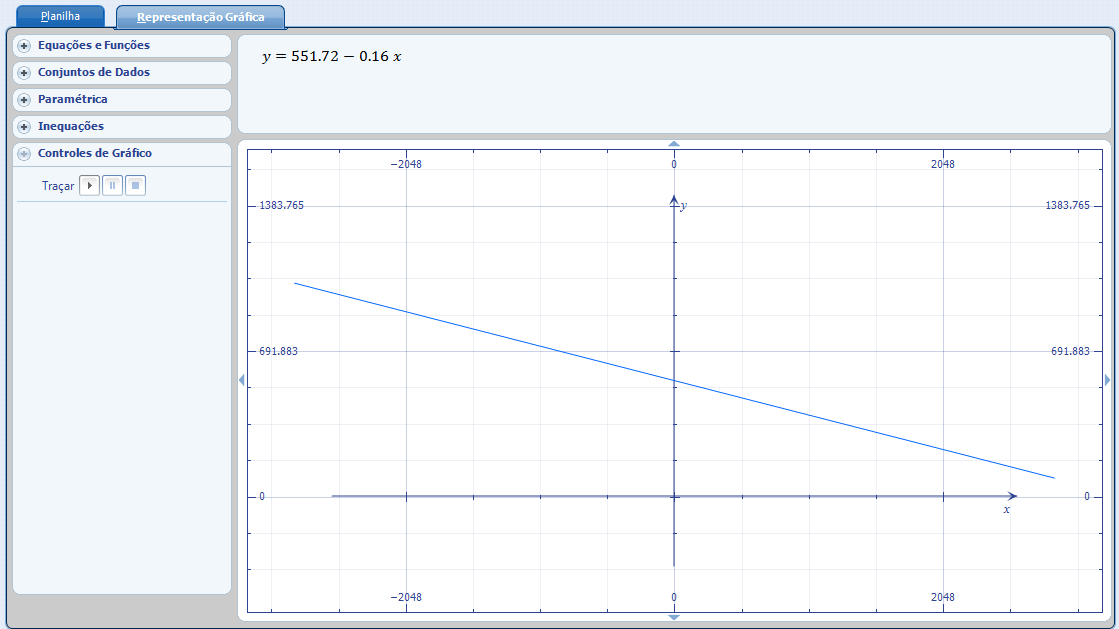
\includegraphics[height=5cm]{imagens/mathematics1.png}
		\caption{Reta analítica correspondente à linha da região demarcada na figura \ref{figMinQuadInterface}}
		\label{mathematics}
	\end{figure}
	
	Com esta técnica se obteve uma possibilidade de automatização da busca de elementos de interesse nas imagens estudadas.
	
	Este aplicativo está disponível em \url{https://github.com/ivancezanne/TCC/tree/master/App_MinimosQuadrados}.
	
	\section{Aplicativo de Projeção 3D}
		\label{app3D}
		
		Tendo em vista que o resultado deste trabalho é gerar malhas 3D, um aplicativo (figura \ref{imagemApp3D}), baseado na descrição presente em \cite{compGraphsPrincPrat3ed} e capaz de interpretar aquivos PLY \cite{ply}, foi desenvolvido. Mesmo apresentando uma limitação quanto a definições de usuário em relação a cores e normais de faces, a utilidade deste aplicativo no contexto deste trabalho foi notável.
		
		\begin{figure}[!htb]
			\centering
			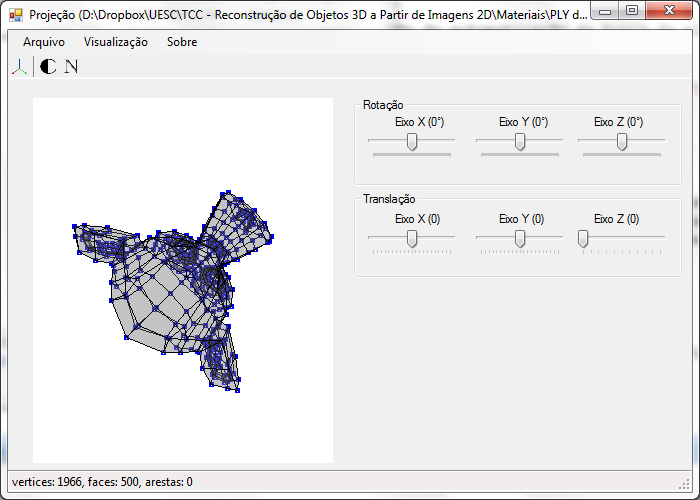
\includegraphics[height=5cm]{imagens/printApp3D.png}
			\caption{Aplicativo de projeção 3D com a famosa malha Suzanne}
			\label{imagemApp3D}
		\end{figure}
		
		Além da projeção da malha 3D descrita em um arquivo PLY de entrada, este aplicativo possibilita manipulações geométricas na malha (translação e rotação, apenas) e algoritmos prontos de normalização (alteração proporcional das dimensões para o máximo de 1 unidade de medida) e centralização (translação do baricentro da malha à origem do espaço 3D).
		
		Como auxílios visuais o aplicativo também permite escolher quais elementos da malha deverão ser projetados à visualização (figura \ref{imagemApp3DRenderizar}) e alterar as cores dos elementos que compõem a malha (figura \ref{imagemApp3DCores}).
		
		\begin{figure}[!htb]
			\centering
			\subfloat[Menu onde se escolhe quais elementos da malha serão renderizados]{
				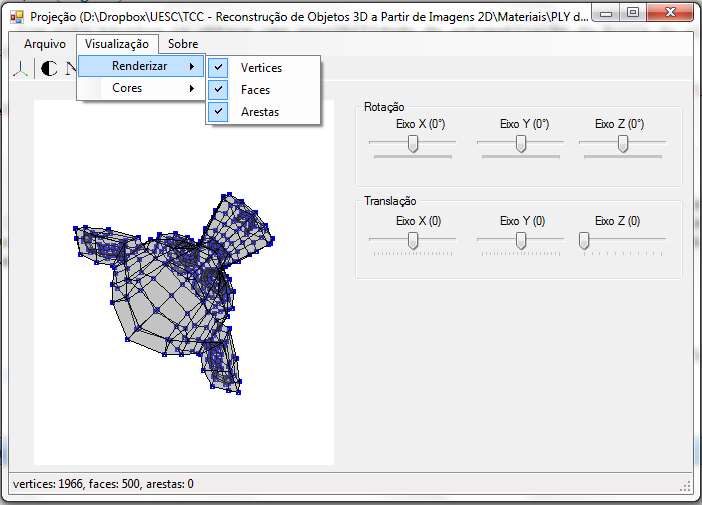
\includegraphics[height=5cm]{imagens/printApp3D-renderizar.png}
				\label{imagemApp3DRenderizar}
			}
			\quad
			\subfloat[Menu onde se pode alterar as cores dos elementos da malha]{
				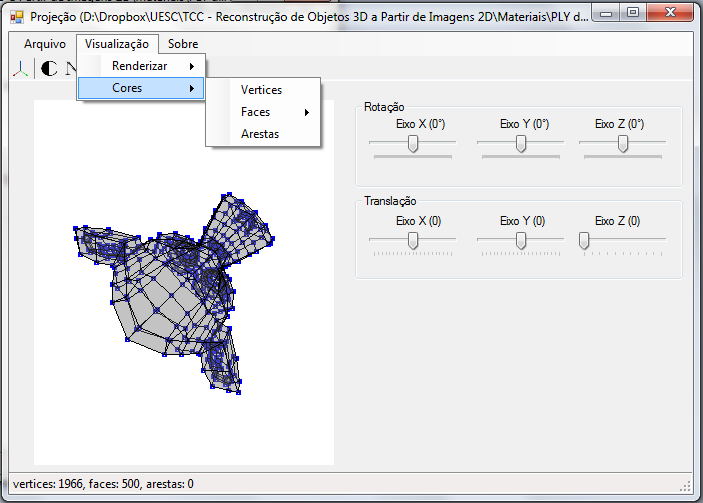
\includegraphics[height=5cm]{imagens/printApp3D-cores.png}
				\label{imagemApp3DCores}
			}
			\caption{Opções adicionais do aplicativo de projeção 3D de auxílio à visualização}
			\label{imagemApp3DAuxiliosVisuais}
		\end{figure}
		
		Por muitas vezes as funcionalidades implementadas neste aplicativo o fizeram preferível, na visualização de resultados deste trabalho, em relação ao \textit{software} MeshLab.
		
		Este aplicativo pode ser encontrado em \url{https://github.com/ivancezanne/TCC/tree/master/App_Projecao}.
		
	\section{Aplicativo de Reconstrução}
		\label{appReconstrucao}
		
		A técnica de reconstrução deste trabalho (capítulo \ref{capituloReconstrucao}) foi implementada através de um \textit{software} (figura \ref{printAppReconstrucao}) que, com forte auxílio visual, busca otimizar a reconstrução almejada.
		
		\begin{figure}[!htb]
			\centering
			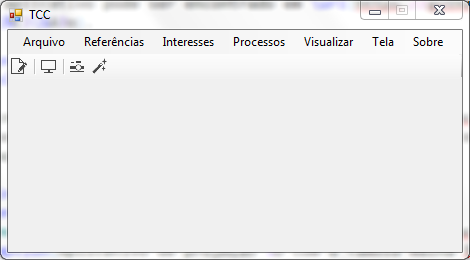
\includegraphics[height=4cm]{imagens/printAppReconstrucao.png}
			\caption{Tela inicial do aplicativo de reconstrução}
			\label{printAppReconstrucao}
		\end{figure}
		
		Inicialmente, o software necessita que uma imagem seja aberta em sua interface para que as demais funcionalidades sejam disponibilizadas. Com uma imagem carregada (que já é aberta com um conjunto de referências arbitrário), a demarcação de pontos de referência e de interesse (capítulo \ref{capituloReconstrucao}) pode ser feita através de \textit{clicks} na região desejada da imagem (figura \ref{printAppReconstrucaoDemarcacao}).
		
		\begin{figure}[!htb]
			\centering
			\subfloat[Interface apenas com uma imagem incial]{
				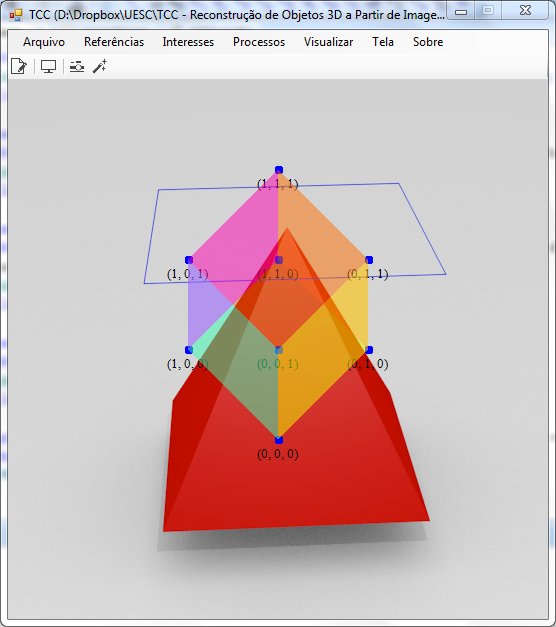
\includegraphics[height=4cm]{imagens/printAppReconstrucaoInicio.png}
				\label{AppReconstrucaoInicio}
			}
			\enskip
			\subfloat[Após o \textit{click}, um \textit{prompt} solicita dados acerca do ponto]{
				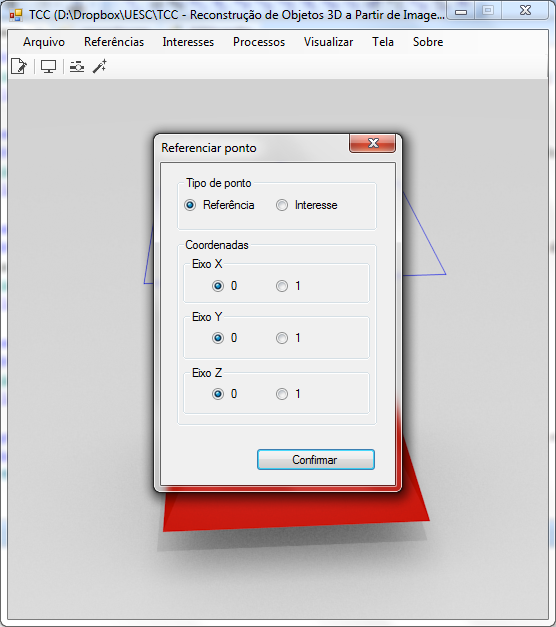
\includegraphics[height=4cm]{imagens/printAppReconstrucaoPrompt.png}
				\label{AppReconstrucaoPrompt}
			}
			\enskip
			\subfloat[Pelos \textit{radio buttons}, o mesmo \textit{prompt} é utilizado para catalogar pontos de referência e de interesse]{
				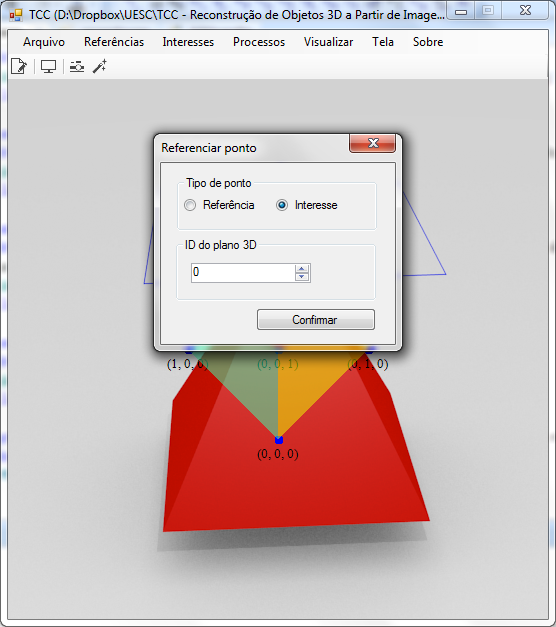
\includegraphics[height=4cm]{imagens/printAppReconstrucaoPromptInteresse.png}
				\label{AppReconstrucaoPromptInteresse}
			}
			\enskip
			\subfloat[Uma cena completamente catalogada]{
				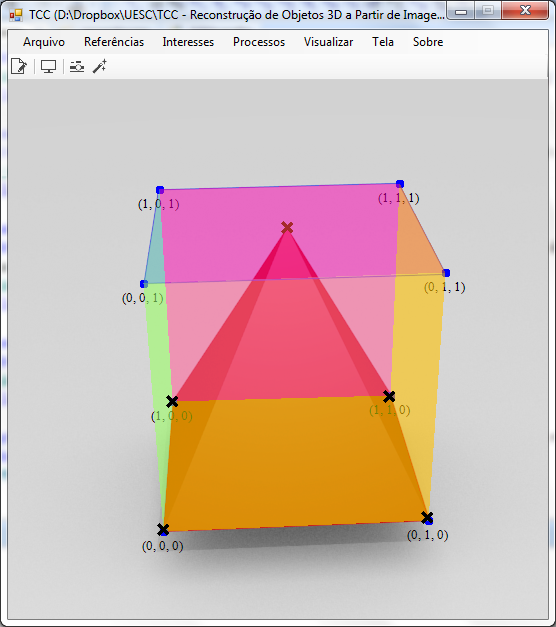
\includegraphics[height=4cm]{imagens/printAppReconstrucaoPronto.png}
				\label{AppReconstrucaoPronto}
			}
			\caption{Utilização da interface para a demarcação de pontos de referência e interesse}
			\label{printAppReconstrucaoDemarcacao}
		\end{figure}
		
		Após o completo fornecimento de dados para a reconstrução, é necessário que se execute a calibração de câmera e só então a reconstrução será possível de ser executada. Para a implementação da calibração foi utilizada o método de cálculo de autovalores e autovetores, baseado no algoritmo QR, da biblioteca ALGLIB Free Edition v3.8.2 para linguagem C\#.
		
		Ao início da reconstrução, os dados descritos no capítulo \ref{capituloReconstrucao} (tolerância projetiva, incremento e critério de convergência) são requisitados pelo software e seu fornecimento é obrigatório ao usuário (figura \ref{printAppReconstrucaoReconstrucao}).
		
		\begin{figure}[!htb]
			\centering
			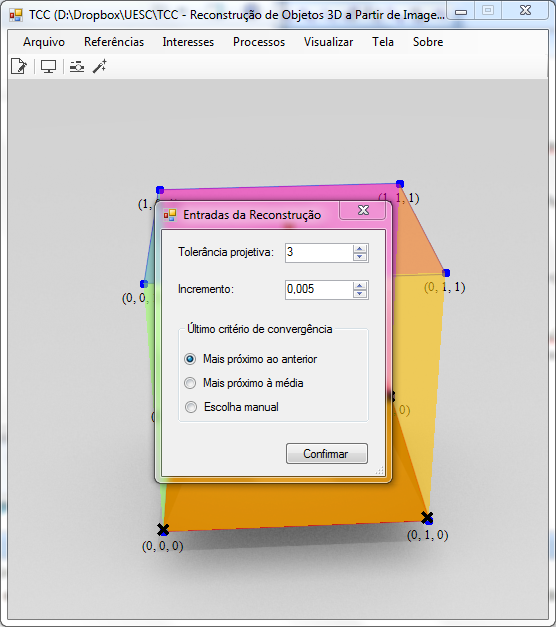
\includegraphics[height=5cm]{imagens/printAppReconstrucaoReconstrucao.png}
			\caption{\textit{Prompt} com dados necessários à reconstrução}
			\label{printAppReconstrucaoReconstrucao}
		\end{figure}
		
		Em adição aos critérios arbitrários de convergência descritos no capítulo \ref{capituloReconstrucao}, o software oferece a possibilidade de escolha manual, pelo usuário, do valor da coordenada Z dentre os que o algoritmo já encontrou como possíveis (figura \ref{printAppReconstrucaoEscolhaManual})
		
		\begin{figure}[!htb]
			\centering
			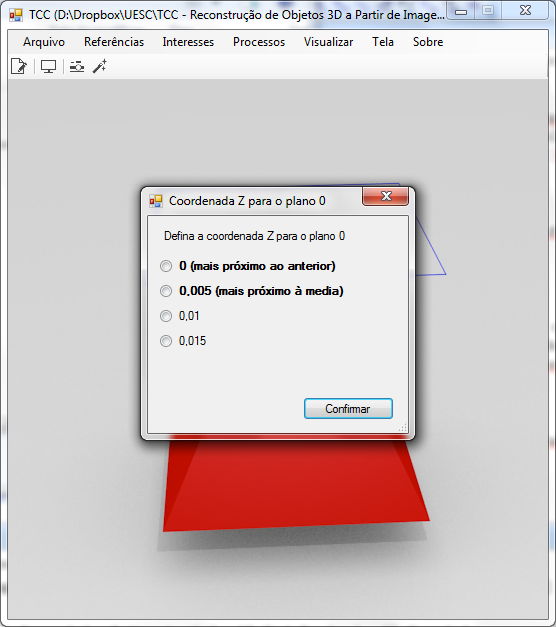
\includegraphics[height=5cm]{imagens/printAppReconstrucaoEscolhaManual.png}
			\caption{\textit{Prompt} para escolha manual da coordenada Z}
			\label{printAppReconstrucaoEscolhaManual}
		\end{figure}
		
		Em posse disto a técnica de reconstrução proposta neste trabalho pode ser executada por qualquer usuário interessado através de um interface adequada. Todavia, ferramentas adicionais como visualização de aproximação após calibração de câmera; salvamento e carregamento de pontos de referência e de interesse através de arquivos; e captura de tela de trabalho foram implementadas tornando o uso do software mais completo e eficiente.
		
		Este aplicativo de reconstrução está disponível em \url{https://github.com/ivancezanne/TCC/tree/master/App_Reconstrucao}.
		
\chapter{Resultados, Discussões e Trabalhos Futuros}
	\label{capituloFinal}
	
	Em posse da técnica descrita no capítulo \ref{capituloReconstrucao} e dos softwares expostos no capítulo \ref{capituloSoftwares}, foi possível obter resultados com certo grau de corretude e com grande potencial de melhora em sua exatidão.
	
	A seguir são apresentados testes, resultados e discussões acerca das atividades desenvolvidas neste trabalho.
	
	\section{Testes validadores}
		\label{secaoTestes}
		
		Como descrito no capítulo \ref{materiaisEMetodos}, a corretude da técnica desenvolvida, e consequente validade dos resultados obtidos, foi aferida através de cenas específicas (figura \ref{cenasValidacao}) cujos dados foram catalogados previamente.
		
		Após alguns testes preliminares, com valores para a tolerância projetiva igual a $3$ e incremento igual a $0.002$, todas as cenas de validação obtiveram seus mais adequados resultados; dependo, individualmente, apenas do critério arbitrário de convergência.
		
		Para a cena de validação 1 (figura \ref{cenaValidacao1}), cuja montagem de dados está expressa na figura \ref{printTesteCubo}, o melhor critério de convergência foi o de valor de coordenada Z mais próximo ao anteriormente analisado.
		
		Demorando, em média, seis minutos e dez segundos para concluir, a reconstrução da cena de validação 1 retornou os dados da tabela \ref{tabelaErrosCubo}.
		
		\begin{table}
			\caption{Dados da reconstrução da cena de validação 1}
			\label{tabelaErrosCubo}
			\begin{center}
				\begin{tabular}{r r r | r r r | r}
					\hline
					\multicolumn{3}{c}{Obtido} & \multicolumn{3}{c}{Desejado}\\
					\cline{1-6}
					\multicolumn{1}{c}{X} & \multicolumn{1}{c}{Y} & \multicolumn{1}{c}{Z} & \multicolumn{1}{c}{X} & \multicolumn{1}{c}{Y} & \multicolumn{1}{c}{Z} & \multicolumn{1}{c}{Erro geométrico}\\
					\hline			
					0.00625				&			0.007035714		&		0				&		0		&		0		&		0		&		0.009410833\\
					0.996142857		&			0.003428571		&		0				&		1		&		0		&		0		&		0.005160683\\
					0.992					&			0.990393443		&		0				&		1		&		1		&		0		&		0.012501438\\
					0.005571429		& 		0.994571429		&		0				&		0		&		1		&		0		&		0.007778831\\
					0.995111111		&			0.005407407		&		0.99		&		1		&		0		&		1		&		0.012375027\\
					0.997					&			0.998					&		0.99		&		1		&		1		&		1		&		0.010630146\\
					0.010571429		&			0.017492063		&		0.99		&		0		&		0		&		1		&		0.022753624\\
					0.009538462		&			0.995461538		&		0.99		&		0		&		1		&		1		&		0.014545786\\
					\hline
				\end{tabular}
			\end{center}
		\end{table}
		
		Na cena de validação 2 (figura \ref{cenaValidacao2}), cuja montagem de dados é a da figura \ref{printTestePiramide}, o critério de convergência mais eficaz, por sua vez, foi o de valor de coordenada Z mais próximo à média dos valores possíveis.
		
		Com uma demora média para conclusão de quatro minutos, a reconstrução da cena 2 retornou os dados da tabela \ref{tabelaErrosPiramide}.
		
		\begin{table}
			\caption{Dados da reconstrução da cena de validação 2}
			\label{tabelaErrosPiramide}
			\begin{center}
				\begin{tabular}{r r r | r r r | r}
					\hline
					\multicolumn{3}{c}{Obtido} & \multicolumn{3}{c}{Desejado}\\
					\cline{1-6}
					\multicolumn{1}{c}{X} & \multicolumn{1}{c}{Y} & \multicolumn{1}{c}{Z} & \multicolumn{1}{c}{X} & \multicolumn{1}{c}{Y} & \multicolumn{1}{c}{Z} & \multicolumn{1}{c}{Erro geométrico}\\
					\hline			
					0.007					&			0.005					&		0.008		&		0			&		0			&		0		&		0.01174734\\
					0.011866667		&			0.99352				&		0.008		&		0			&		1			&		0		&		0.01571013\\
					0.9675671			&			0.989264069		&		0.008		&		1			&		1			&		0		&		0.035087793\\
					0.982966292		& 		0.004876404		&		0.008		&		1			&		0			&		0		&		0.019440332\\
					0.766722973		&			0.517574324		&		0.904		&		0.5		&		0.5		&		1		&		0.284017607\\
					\hline
				\end{tabular}
			\end{center}
		\end{table}
		
		Na cena de validação 3 (figura \ref{cenaValidacao3}) - montagem da figura \ref{printTesteCuboReduzido}, novamente, o critério de escolher coordenadas Z cujo valor é mais próximo ao plano analisado anteriormente foi o melhor.
		
		Em média, eram gastos seis minutos e vinte segundos para a reconstrução da cena de validação 3 retornar os dados da tabela \ref{tabelaErrosCuboReduzido}.
		
		\begin{table}
			\caption{Dados da reconstrução da cena de validação 3}
			\label{tabelaErrosCuboReduzido}
			\begin{center}
				\begin{tabular}{r r r | r r r | r}
					\hline
					\multicolumn{3}{c}{Obtido} & \multicolumn{3}{c}{Desejado}\\
					\cline{1-6}
					\multicolumn{1}{c}{X} & \multicolumn{1}{c}{Y} & \multicolumn{1}{c}{Z} & \multicolumn{1}{c}{X} & \multicolumn{1}{c}{Y} & \multicolumn{1}{c}{Z} & \multicolumn{1}{c}{Erro geométrico}\\
					\hline			
					0.507521739		&			0.512478261		&		0				&		0.5			&		0.5			&		0			&		0.014569954\\
					0.504075949		&			0.992075949		&		0				&		0.5			&		1				&		0			&		0.008910889\\
					0.989418182		&			0.511109091		&		0				&		1				&		0.5			&		0			&		0.01534232\\
					0.98727027		& 		0.981310811		&		0				&		1				&		1				&		0			&		0.022612647\\
					0.521545455		&			0.521545455		&		0.492		&		0.5			&		0.5			&		0.5		&		0.031502591\\
					0.511					&			0.99575				&		0.492		&		0.5			&		1				&		0.5		&		0.01425\\
					0.9972 				&			0.5164				&		0.492		&		1				&		0.5			&		0.5		&		0.018460769\\
					0.996181818		&			0.995454545		&		0.492		&		1				&		1				&		0.5		&		0.009961911\\
					\hline	
				\end{tabular}
			\end{center}
		\end{table}	
		
		
		
		\begin{figure}[!htb]
			\centering
			\subfloat[Panorama para a reconstrução da cena de validação 1]{
				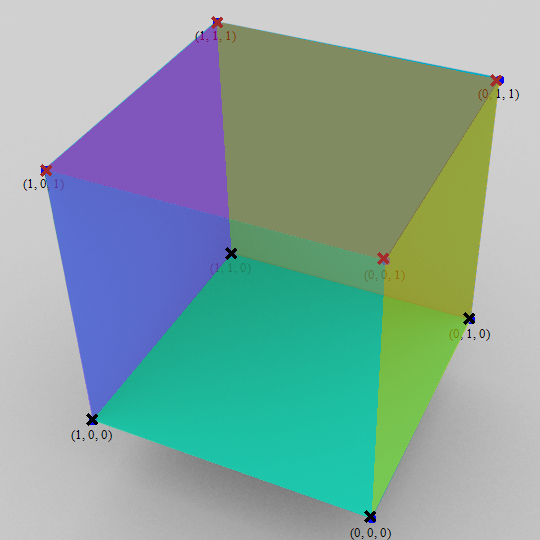
\includegraphics[height=4.5cm]{imagens/printTesteCubo.png}
				\label{printTesteCubo}
			}
			\quad
			\subfloat[Panorama da reconstrução da cena de validação 2]{
				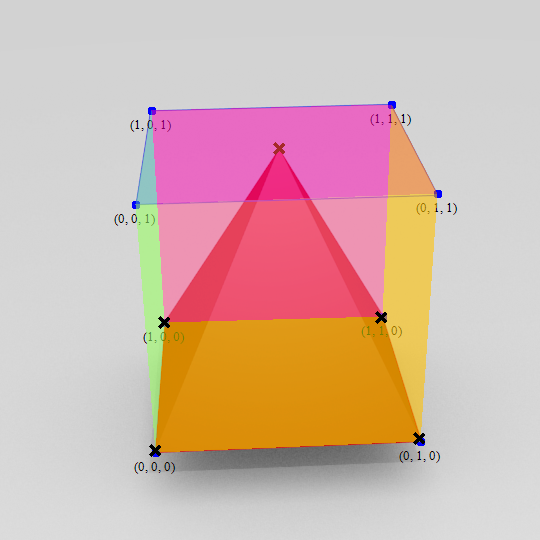
\includegraphics[height=4.5cm]{imagens/printTestePiramide.png}
				\label{printTestePiramide}
			}
			\quad
			\subfloat[Panorama da reconstrução da cena de validação 3]{
				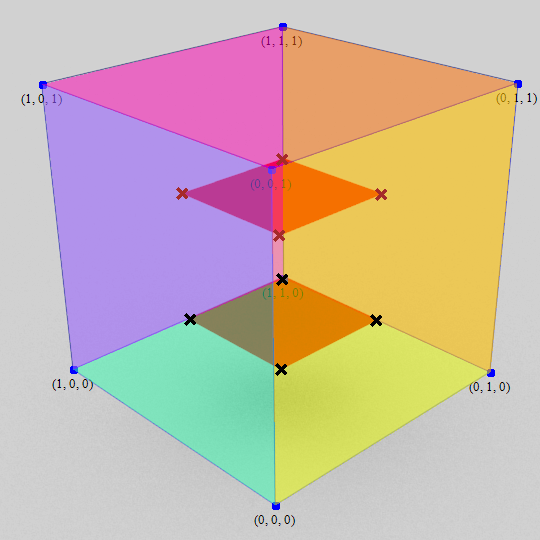
\includegraphics[height=4.5cm]{imagens/printTesteCuboReduzido.png}
				\label{printTesteCuboReduzido}
			}
			\caption{Panoramas das reconstruções de validação}
			\label{printTestes}
		\end{figure}
		
		Através da escolha manual, disponibilizada pelo aplicativo de reconstrução, de valores para as coordenadas Z, há um erro geométrico médio menor entre os pontos, fazendo com que a geometria dos objetos reconstruídos seja mais verossímil. Todavia, a escolha manual é uma estratégia notavelmente brusca e, por isso, resolveu-se não discuti-la nesta monografia.
		
		Todos os dados e resultados dos testes validadores, inclusive os correspondentes à escolha manual, estão disponíveis em \url{https://github.com/ivancezanne/TCC/tree/master/App_Reconstrucao/Testes}.
		
		\section{Resultados}
			\label{secaoResultados}
			
		\section{Discussões}
			\label{secaoDiscussoes}
			
		\section{Trabalhos Futuros}
			\label{secaoTrabalhosFuturos}

%-----------Bibliografia------------------------------------

%\nocite{*}

%\bibliographystyle{bst/abntex2-alf}

\bibliography{bibliografia} % arquivos com as entradas bib.

\end{document}
